% Options for packages loaded elsewhere
\PassOptionsToPackage{unicode}{hyperref}
\PassOptionsToPackage{hyphens}{url}
\PassOptionsToPackage{dvipsnames,svgnames,x11names}{xcolor}
%
\documentclass[
  oneclumn]{article}

\usepackage{amsmath,amssymb}
\usepackage{iftex}
\ifPDFTeX
  \usepackage[T1]{fontenc}
  \usepackage[utf8]{inputenc}
  \usepackage{textcomp} % provide euro and other symbols
\else % if luatex or xetex
  \usepackage{unicode-math}
  \defaultfontfeatures{Scale=MatchLowercase}
  \defaultfontfeatures[\rmfamily]{Ligatures=TeX,Scale=1}
\fi
\usepackage{lmodern}
\ifPDFTeX\else  
    % xetex/luatex font selection
\fi
% Use upquote if available, for straight quotes in verbatim environments
\IfFileExists{upquote.sty}{\usepackage{upquote}}{}
\IfFileExists{microtype.sty}{% use microtype if available
  \usepackage[]{microtype}
  \UseMicrotypeSet[protrusion]{basicmath} % disable protrusion for tt fonts
}{}
\makeatletter
\@ifundefined{KOMAClassName}{% if non-KOMA class
  \IfFileExists{parskip.sty}{%
    \usepackage{parskip}
  }{% else
    \setlength{\parindent}{0pt}
    \setlength{\parskip}{6pt plus 2pt minus 1pt}}
}{% if KOMA class
  \KOMAoptions{parskip=half}}
\makeatother
\usepackage{xcolor}
\usepackage[left=35mm,right=35mm,top=15mm,bottom=20mm,noheadfoot]{geometry}
\setlength{\emergencystretch}{3em} % prevent overfull lines
\setcounter{secnumdepth}{-\maxdimen} % remove section numbering
% Make \paragraph and \subparagraph free-standing
\ifx\paragraph\undefined\else
  \let\oldparagraph\paragraph
  \renewcommand{\paragraph}[1]{\oldparagraph{#1}\mbox{}}
\fi
\ifx\subparagraph\undefined\else
  \let\oldsubparagraph\subparagraph
  \renewcommand{\subparagraph}[1]{\oldsubparagraph{#1}\mbox{}}
\fi


\providecommand{\tightlist}{%
  \setlength{\itemsep}{0pt}\setlength{\parskip}{0pt}}\usepackage{longtable,booktabs,array}
\usepackage{calc} % for calculating minipage widths
% Correct order of tables after \paragraph or \subparagraph
\usepackage{etoolbox}
\makeatletter
\patchcmd\longtable{\par}{\if@noskipsec\mbox{}\fi\par}{}{}
\makeatother
% Allow footnotes in longtable head/foot
\IfFileExists{footnotehyper.sty}{\usepackage{footnotehyper}}{\usepackage{footnote}}
\makesavenoteenv{longtable}
\usepackage{graphicx}
\makeatletter
\def\maxwidth{\ifdim\Gin@nat@width>\linewidth\linewidth\else\Gin@nat@width\fi}
\def\maxheight{\ifdim\Gin@nat@height>\textheight\textheight\else\Gin@nat@height\fi}
\makeatother
% Scale images if necessary, so that they will not overflow the page
% margins by default, and it is still possible to overwrite the defaults
% using explicit options in \includegraphics[width, height, ...]{}
\setkeys{Gin}{width=\maxwidth,height=\maxheight,keepaspectratio}
% Set default figure placement to htbp
\makeatletter
\def\fps@figure{htbp}
\makeatother

\usepackage{inputenc}
\makeatletter
\@ifpackageloaded{caption}{}{\usepackage{caption}}
\AtBeginDocument{%
\ifdefined\contentsname
  \renewcommand*\contentsname{Table of contents}
\else
  \newcommand\contentsname{Table of contents}
\fi
\ifdefined\listfigurename
  \renewcommand*\listfigurename{List of Figures}
\else
  \newcommand\listfigurename{List of Figures}
\fi
\ifdefined\listtablename
  \renewcommand*\listtablename{List of Tables}
\else
  \newcommand\listtablename{List of Tables}
\fi
\ifdefined\figurename
  \renewcommand*\figurename{Figure}
\else
  \newcommand\figurename{Figure}
\fi
\ifdefined\tablename
  \renewcommand*\tablename{Table}
\else
  \newcommand\tablename{Table}
\fi
}
\@ifpackageloaded{float}{}{\usepackage{float}}
\floatstyle{ruled}
\@ifundefined{c@chapter}{\newfloat{codelisting}{h}{lop}}{\newfloat{codelisting}{h}{lop}[chapter]}
\floatname{codelisting}{Listing}
\newcommand*\listoflistings{\listof{codelisting}{List of Listings}}
\makeatother
\makeatletter
\makeatother
\makeatletter
\@ifpackageloaded{caption}{}{\usepackage{caption}}
\@ifpackageloaded{subcaption}{}{\usepackage{subcaption}}
\makeatother
\ifLuaTeX
  \usepackage{selnolig}  % disable illegal ligatures
\fi
\usepackage{bookmark}

\IfFileExists{xurl.sty}{\usepackage{xurl}}{} % add URL line breaks if available
\urlstyle{same} % disable monospaced font for URLs
\hypersetup{
  colorlinks=true,
  linkcolor={blue},
  filecolor={Maroon},
  citecolor={Blue},
  urlcolor={Blue},
  pdfcreator={LaTeX via pandoc}}

\author{}
\date{2024-10-31}

\begin{document}

\section{Universidade Federal de
Pernambuco}\label{universidade-federal-de-pernambuco}

\vspace{-.4cm}

\section{Centro de Ciências Exatas e da
Natureza}\label{centro-de-ciuxeancias-exatas-e-da-natureza}

\vspace{-.4cm}

\section{Departamento de
Estatística}\label{departamento-de-estatuxedstica}

\vspace{.5cm}

\subsection{TÓPICOS ESPECIAIS EM ESTATÍSTICA
COMPUTACIONAL}\label{tuxf3picos-especiais-em-estatuxedstica-computacional}

\vspace{.5cm}

\textbf{Data:} 21 de março de 2025

\vspace{.5cm}

\section{Introdução}\label{introduuxe7uxe3o}

Prever possíveis falhas em máquinas e equipamentos industriais é uma
ótima forma de combater um dos problemas mais recorrentes em empresas.
Quando um equipamento falha ele pode acarretar vários problemas que
podem gerar problemas de produção, acidentes e grandes percas
financeiras, e a melhor forma de evitar isso é prevenindo esses erros.
Com isso, esse trabalho tem como objetivo buscar um forma de prever
essas falhas através de modelos de predição com aprendizado de máquina
utilizando dados sintéticos reflete a manutenção preditiva real
encontrada no setor, onde são apresentados variáveis que possam nos
ajudar a chegar o mais próximo do resultado desejado e aumentar o máximo
possível a possibilidade de evitar as falhas nas maquinas.

\section{Fundamentos Teóricos e
Metodológicos}\label{fundamentos-teuxf3ricos-e-metodoluxf3gicos}

O conjunto de dados utilizado nesse projeto se chama ``Explainable
Artificial Intelligence for Predictive Maintenance Applications'' e é
composto por 14 variáveis e 10.000 observações. Foi utilizada a
linguagem Python para obter as análises e a aplicação dos modelos de
Árvore de Decisão e Floresta Aleatória, a variável de classificação é a
variável binária ``Target'' que apresenta 0 para as observações que a
maquina apresentou falha e 1 para as que não apresentaram falha.

\subsubsection{Variáveis utilizadas:}\label{variuxe1veis-utilizadas}

\begin{itemize}
\item
  \textbf{UID}: identificador único que varia de 1 a 10000.
\item
  \textbf{productID}: consistindo em uma letra L, M ou H para baixo
  (50\% de todos os produtos), médio (30\%) e alto (20\%) como variantes
  de qualidade do produto e um número de série específico da variante.
\item
  \textbf{Type}: Apresenta somente as variantes de qualidade de produto
  (L, M e H).
\item
  \textbf{air temperature {[}K{]}}: gerada usando um processo de
  caminhada aleatória posteriormente normalizada para um desvio padrão
  de 2 K em torno de 300 K.
\item
  \textbf{process temperature {[}K{]}}: gerada usando um processo de
  caminhada aleatória normalizado para um desvio padrão de 1 K,
  adicionado à temperatura do ar mais 10 K.
\item
  \textbf{rotational speed {[}rpm{]}}: calculada a partir da potência de
  2860 W, sobreposta com um ruído normalmente distribuído.
\item
  \textbf{torque {[}Nm{]}}: os valores de torque são normalmente
  distribuídos em torno de 40 Nm com um σ = 10 Nm e sem valores
  negativos.
\item
  \textbf{tool wear {[}min{]}}: As variantes de qualidade H/M/L
  adicionam 5/3/2 minutos de desgaste da ferramenta à ferramenta usada
  no processo.
\item
  \textbf{Failure Type}: Indica o tipo de falha da máquina. Não
  utilizamos essa variável pois também é uma variável de classificação.
\end{itemize}

\section{Aplicação}\label{aplicauxe7uxe3o}

De início vamos apresentar a analise exploratória dos dados para que
possamos entender como os dados a distribuição dos dados de cada
variável presente no conjunto de dados.

\subsubsection{Análise Exploratória}\label{anuxe1lise-exploratuxf3ria}

\begin{longtable}[]{@{}
  >{\raggedright\arraybackslash}p{(\columnwidth - 10\tabcolsep) * \real{0.0777}}
  >{\raggedleft\arraybackslash}p{(\columnwidth - 10\tabcolsep) * \real{0.1942}}
  >{\raggedleft\arraybackslash}p{(\columnwidth - 10\tabcolsep) * \real{0.2330}}
  >{\raggedleft\arraybackslash}p{(\columnwidth - 10\tabcolsep) * \real{0.2233}}
  >{\raggedleft\arraybackslash}p{(\columnwidth - 10\tabcolsep) * \real{0.1165}}
  >{\raggedleft\arraybackslash}p{(\columnwidth - 10\tabcolsep) * \real{0.1553}}@{}}
\caption{Medidas descritivas das variáveis númericas}\tabularnewline
\toprule\noalign{}
\begin{minipage}[b]{\linewidth}\raggedright
Medida
\end{minipage} & \begin{minipage}[b]{\linewidth}\raggedleft
Air temperature {[}K{]}
\end{minipage} & \begin{minipage}[b]{\linewidth}\raggedleft
Process temperature {[}K{]}
\end{minipage} & \begin{minipage}[b]{\linewidth}\raggedleft
Rotational speed {[}rpm{]}
\end{minipage} & \begin{minipage}[b]{\linewidth}\raggedleft
Torque {[}Nm{]}
\end{minipage} & \begin{minipage}[b]{\linewidth}\raggedleft
Tool wear {[}min{]}
\end{minipage} \\
\midrule\noalign{}
\endfirsthead
\toprule\noalign{}
\begin{minipage}[b]{\linewidth}\raggedright
Medida
\end{minipage} & \begin{minipage}[b]{\linewidth}\raggedleft
Air temperature {[}K{]}
\end{minipage} & \begin{minipage}[b]{\linewidth}\raggedleft
Process temperature {[}K{]}
\end{minipage} & \begin{minipage}[b]{\linewidth}\raggedleft
Rotational speed {[}rpm{]}
\end{minipage} & \begin{minipage}[b]{\linewidth}\raggedleft
Torque {[}Nm{]}
\end{minipage} & \begin{minipage}[b]{\linewidth}\raggedleft
Tool wear {[}min{]}
\end{minipage} \\
\midrule\noalign{}
\endhead
\bottomrule\noalign{}
\endlastfoot
Min. & 295.3 & 305.7 & 1168 & 3.80 & 0 \\
1st Qu. & 298.3 & 308.8 & 1423 & 33.20 & 53 \\
Median & 300.1 & 310.1 & 1503 & 40.10 & 108 \\
Mean & 300.0 & 310.0 & 1539 & 39.99 & 108 \\
3rd Qu. & 301.5 & 311.1 & 1612 & 46.80 & 162 \\
Max. & 304.5 & 313.8 & 2886 & 76.60 & 253 \\
\end{longtable}

\begin{figure}[H]

{\centering 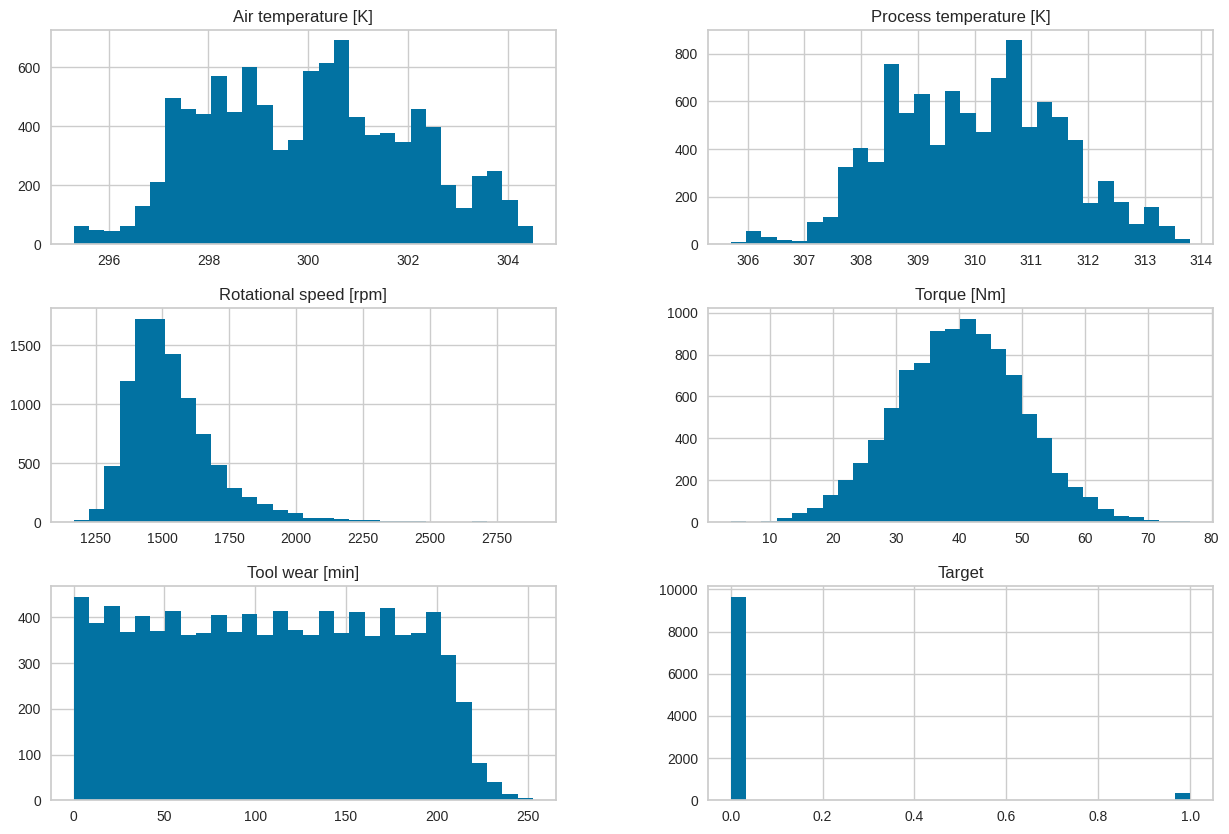
\includegraphics{graficos.png}

}

\caption{Gráficos com de distribuição das variáveis númericas}

\end{figure}%

Na \textbf{Table 1} podemos observar que as variáveis \emph{``Air
temperature {[}K{]}''} e \emph{``Process temperature {[}K{]}''}
apresentam baixa variação na distribuição dos dados quando observamos os
quartis, já as demais variáveis possuem grande variação, todas essas
afirmações podem ser observadas na \textbf{Figure 1}.

\begin{figure}[H]

{\centering 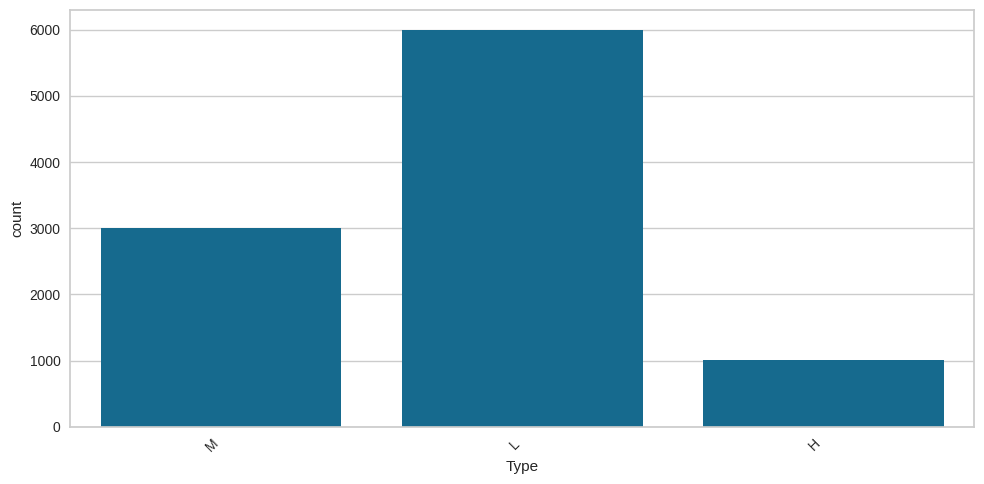
\includegraphics[width=0.8\textwidth,height=\textheight]{graficos_categoricas.png}

}

\caption{Gráfico com a distribuição da váriavel ``Type''}

\end{figure}%

A única variável categórica que temos no conjunto de dados é a várivavel
\emph{''Type''} que classifica os produtos por qualidade, sendo L para
baixa qualidade, M para média qualidade e H para Alta qualidade. Na
\textbf{Figure 2} podemos ver que as maquinas de baixa qualidade são as
mais presentes nos dados.

\newpage

\subsubsection{Aplicação do modelo}\label{aplicauxe7uxe3o-do-modelo}

Para essa estudo escolhemos os modelos de \textbf{Árvore de decisão} e
\textbf{Floresta aleatória} para comparar qual modelo apresenta melhor
desempenho resolver nosso problema.

\begin{figure}

\begin{minipage}{0.50\linewidth}

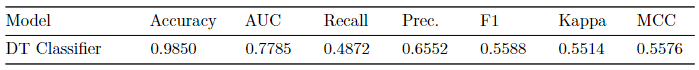
\includegraphics{dt_table.png}

\subcaption{\label{}Métricas do modelo de Árvore de decisão}
\end{minipage}%
%
\begin{minipage}{0.50\linewidth}

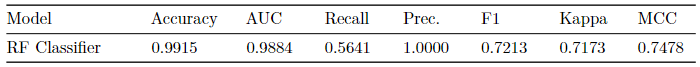
\includegraphics{rf_table.png}

\subcaption{\label{}Métricas do modelo de Floresta Aleatória}
\end{minipage}%
\newline
\begin{minipage}{0.50\linewidth}

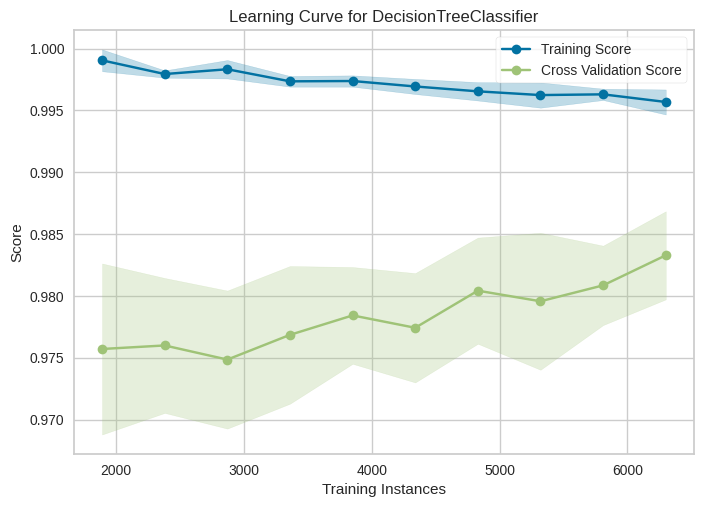
\includegraphics{dt_learn.png}

\subcaption{\label{}Curva de aprendizado da Árvore de decisão}
\end{minipage}%
%
\begin{minipage}{0.50\linewidth}

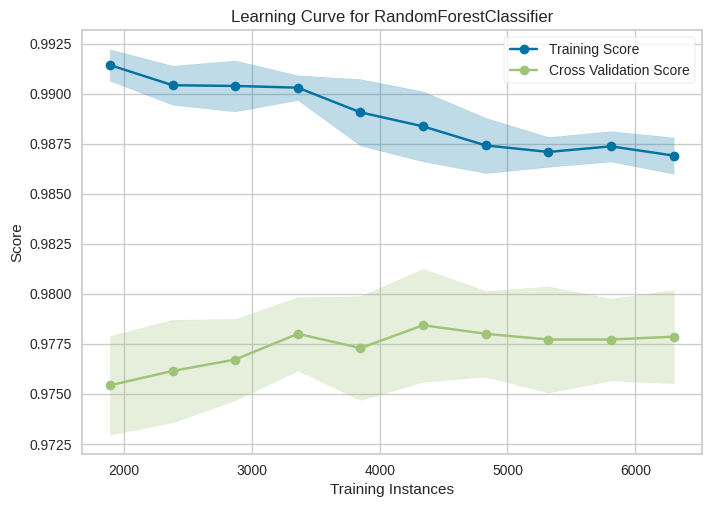
\includegraphics{rf_learn.png}

\subcaption{\label{}Curva de aprendizado da Floresta Aleatória}
\end{minipage}%
\newline
\begin{minipage}{0.50\linewidth}

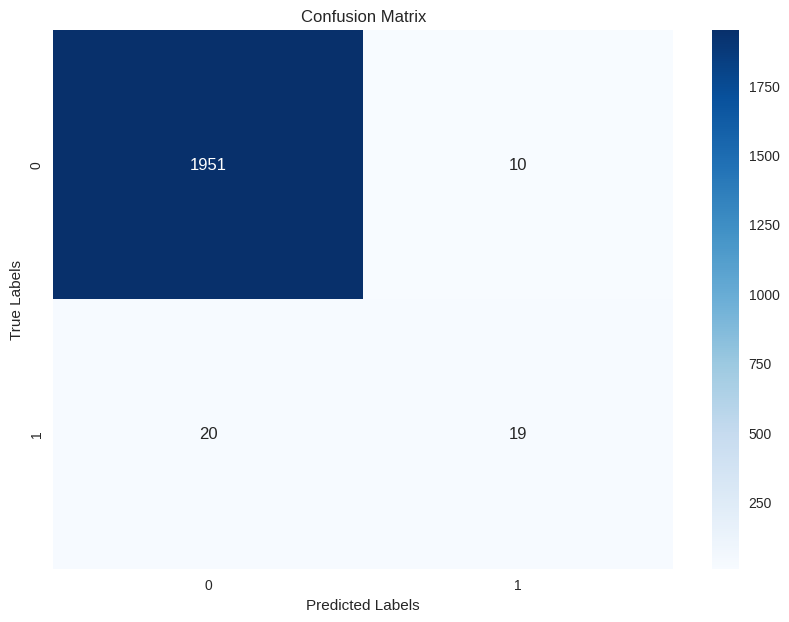
\includegraphics{mc_dt.png}

\subcaption{\label{}Matriz de confusão da Árvore de decisão}
\end{minipage}%
%
\begin{minipage}{0.50\linewidth}

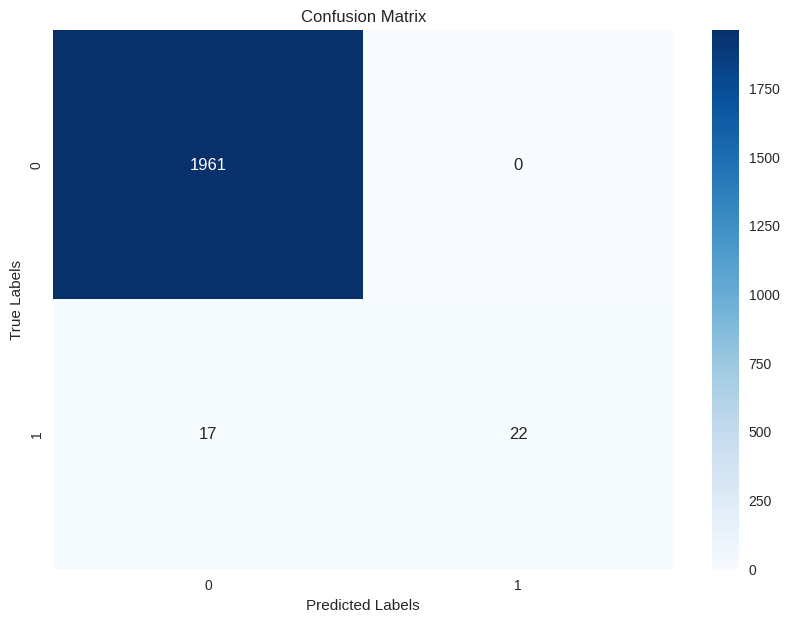
\includegraphics{mc_rf.png}

\subcaption{\label{}Matriz de confusão da Floresta Aleatória}
\end{minipage}%

\end{figure}%

Nas imagens acima podemos ver que o modelo que apresentou melhor
desempenho foi o modelo de árvore aleatória, isso pode ser influenciado
pela dimensão dos dados já que o modelo tem melhor desempenho para
grandes quantidades de observações se comparado com o modelo de árvores
de decisão. Nas matrizes de confusão podemos observar que apesar do
desempenho da floresta aleatória se sobressair em relação a árvore de
decisão, podemos que o modelo obteve um resultado muito baixo para
classificar as máquinas com falha, identificando apensa 56\% das
máquinas.

\newpage

\section{Conclusão}\label{conclusuxe3o}

Nesse estudo utilizamos os dados em modelos de classificação e tentamos
chegar ao melhor resultado possível comparando esses dois modelos e
observando o desempenho de ambos para encontrarmos uma forma de
classificar maquinas com possíveis futuras falhas com objetivo de
diminuir problemas nas empresas.

Vimos que modelo de floresta aleatória obteve um resultado melhor se
comparado com o resultado do modelo de árvore de decisão, contudo, não
podemos considerar esse resultado o melhor possível podemos pensar: Qual
foi o problema?

Mesmo com a grande quantidade de observações e variáveis que utilizamos,
podemos perceber que os resultados não apresentaram a melhor performance
possível dos modelos, contudo tivemos a oportunidade de comparar o
desempenho dos dois modelos se testados com o mesmo conjunto de dados e
observar suas performances.

\section{Contribuição da equipe}\label{contribuiuxe7uxe3o-da-equipe}

\begin{itemize}
\tightlist
\item
  \emph{Edgar Carlos Rodrigue de Oliveira:} Fez a ànalise exploratória e
  aplicou o modelo de árvore aleatória (50\% de contribuição).
\item
  \emph{Vitória Karolinny dos Santos Gonçalves:} Aplicou o modelo de
  Floresta Aleatória e criou o relatório e slide (50\% de contribuição).
\end{itemize}

\section{Referências}\label{referuxeancias}

\begin{itemize}
\tightlist
\item
  Link para ter acesso aos dados:
  https://archive.ics.uci.edu/dataset/601/ai4i+2020+predictive+maintenance+dataset
\end{itemize}



\end{document}
